\section{Introduction}
On a long downgrade, a heavy-duty vehicle must coordinate service and auxiliary brakes as friction heating reduces service-brake authority. A leader disturbance can simultaneously raise collision-avoidance demand before either actuator reaches its commanded force. The vehicle-control question is whether \emph{any} admissible pair of brake commands remains, not merely whether a nominal tracking command can be filtered. In a platoon, one thermally constrained vehicle can become the upstream safety bottleneck. Figure~\ref{fig:framework} links this physical conflict to command geometry, feasibility monitoring, and verified execution; its lower strip is training-only.

Heavy-vehicle brake and thermal models \cite{nhtsa2010scam,talati2009brake}, downhill dual-brake allocation \cite{li2025retarder}, brake-fade-aware platooning \cite{devika2022fade}, cooperative cruise control \cite{naus2010string,ploeg2011cacc}, and control barrier function (CBF) quadratic programs (QPs) \cite{ames2017cbf,xiao2022hocbf} address parts of this problem. None directly gives the compact, exact command-feasibility test for simultaneous collision demand, thermal fade, and lagged, gear/power-limited auxiliary braking developed here.

The hard QP has exactly two decision variables, friction command $u_i^f$ and auxiliary command $u_i^a$. Jerk is a post-action comfort metric, not a slack or decision variable. The certificate depends on the hard set rather than the nominal command, which may be supplied by a learned policy, model-predictive controller, or cooperative cruise controller.

The vehicle-control contributions are:
\begin{itemize}
\item \emph{Physical command geometry:} combine friction thermal/fade limits, auxiliary availability, actuator dynamics, collision demand, and an undivided low-speed thermal row in a two-command hard set.
\item \emph{Exact instantaneous certificate:} construct $\rho_i\ge0$ if and only if that hard set is nonempty, with normalized attribution to friction, auxiliary, collision, or low-speed state limitations, independently of the nominal controller.
\item \emph{Predictive and connected-vehicle monitoring:} derive a one-sided finite-horizon certificate under sound enclosure and an age-aware recursive vehicle-to-vehicle bottleneck with vehicle, horizon, and physical-limit attribution. The evaluated floating-point predictor remains a numerical monitor.
\item \emph{Verified supervision and validation:} coordinate four dual-brake supervisory modes and reverify changed commands; model-based boundary and matched comparisons distinguish available brake authority from closed-loop benefit.
\end{itemize}

Negative predictive values do not prove future infeasibility, and delayed upstream values are not instantaneous fleet-global truth. Differentiation through the QP is a secondary learning diagnostic.

\begin{figure*}[t]
\centering
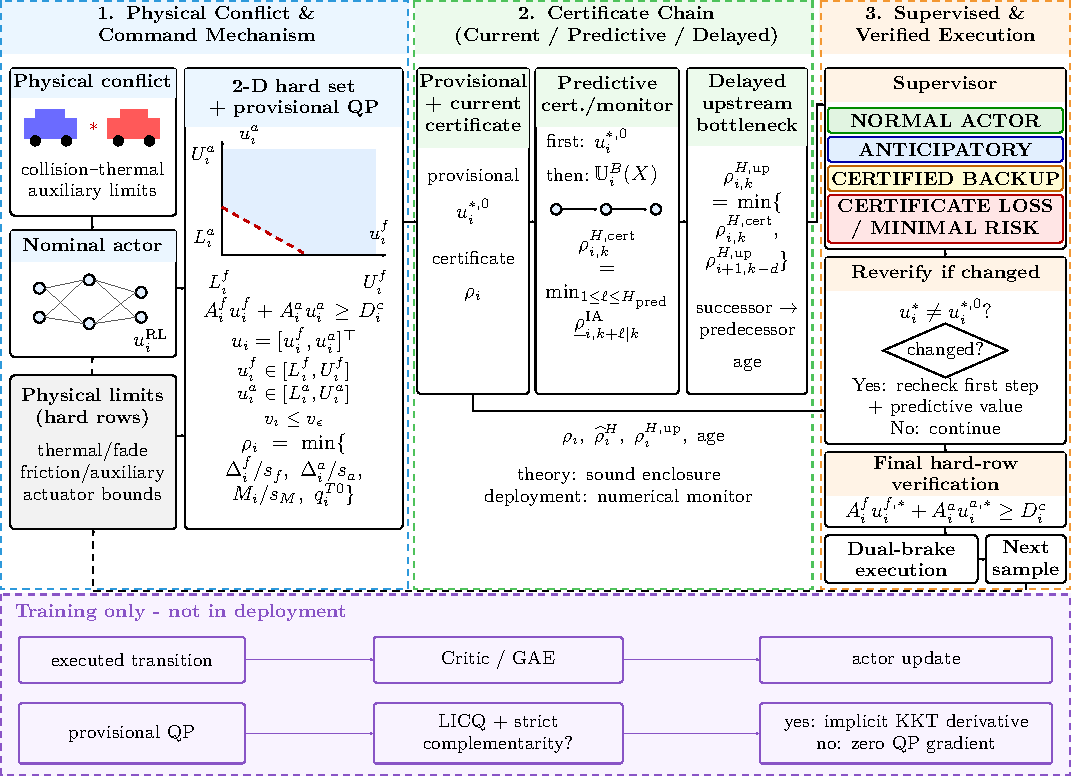
\includegraphics[width=\textwidth]{figures/fig1_desktop66_final.pdf}
\caption{Certificate-aware dual-brake command mechanism. Collision demand and physical limits define the two-dimensional hard set and instantaneous reserve. The theoretical predictive certificate $\rho_{i,k}^{H,{\rm cert}}$ requires sound enclosure; deployment uses the numerical monitor $\widehat{\rho}_{i,k}^{H}$, whose negative value is a warning only. The displayed upstream recursion is theoretical; deployment aggregates age-delayed numerical values for four-mode supervision. A changed action is reverified, and all hard rows are checked before execution. The lower strip denotes training-only secondary diagnostics.}
\label{fig:framework}
\end{figure*}
